\documentclass[12pt]{article}
\usepackage[margin=1in]{geometry}
\usepackage{color}   %May be necessary if you want to color links
\usepackage{hyperref}
\usepackage{setspace}
\usepackage{float}
\usepackage{ulem}
\doublespacing
\hypersetup{
    colorlinks=true, %set true if you want colored links
    linktoc=all,     %set to all if you want both sections and subsections linked
    linkcolor=blue,  %choose some color if you want links to stand out
}
\usepackage{graphicx}
\graphicspath{ {../../images/} }
\setlength{\belowcaptionskip}{-10pt}
\setlength{\abovecaptionskip}{-10pt}
\begin{document}

%a) Title Page - Project title, project adviser, semester, and year.
\begin{titlepage}
	\begin{center}
		\vspace{20pt}
		{\bf \LARGE Indoor Micro-UAV Navigation with Minimal Sensing} \\
		\vspace{200pt}
		Dennis Melamed\footnote{University of Minnesota, Department of Electrical and Computer Engineering} \\
		Advisers: Professor Volkan Isler\footnote{University of Minnesota, Department of Computer Science and Engineering} \& Professor Derya Aksaray\footnote{University of Minnesota, Department of Aerospace Engineering and Mechanics} \\
		Progress Report for Senior Honors Design Project (EE 4982V)\\
		Spring 2018 \\
	\end{center}
\end{titlepage}


%A 200-300 word abstract clearly summarizing the problem being investigated, why this is an interesting problem, the methodology being used, and the progress to date.
\begin{abstract}
    The usage of a small UAV (unmanned aerial vehicle) with minimal sensing abilities to navigate complex indoor environments outside a motion capture system has not been well explored. This work reports on progress in developing a framework to fly out the door of a room from an arbitrary initial location using a micro-UAV with low-accuracy sensors. The sensing abilities will be limited by the payload of the UAV to a low-resolution camera and a low-accuracy IMU. The framework will consist of several interacting components: door detection (by a simple Hough transform procedure or a convolutional neural network), flight planning (via dead reckoning, a recurrent neural network, or a reinforcement learning network), and a lower level flight controller. The methods for door detection have been written and analyzed, with the convolutions neural network model showing significant advantages over the Hough transform based method. Some work still remains to make them usable. Initial groundwork for flight planning is also nearing completion, with a stable UAV payload designed and test flights completed. 
\end{abstract}

%c) Table of Contents - List and page numbers of the different sections.
\tableofcontents

%d) List of Figures - Figure numbers, figure captions, and page numbers.
\listoffigures

%An introduction summarizing the project and an explanation of its importance.
\section{Introduction}
Most current work in the field of autonomous unmanned aerial vehicles (UAVs) uses well-known localization systems such as GPS, motion capture systems, or on-board sensor fusion to determine the UAV's position and orientation. While these systems are reasonable in certain situations, they each have key drawbacks. GPS devices are heavy and can be inaccurate by several meters depending on the location and model of GPS. Motion capture systems are expensive to install and only allow localization within a small area. Sensor fusion on-board the UAV runs into the same problems as GPS, with accuracy often being relatively poor depending on the environment and sensors used. Weight is an additional concern, as cameras and others sensors sufficient to give good sensor fusion can often weigh more than the payload of the UAV. Due to these issues, it is desirable to find a way a lightweight UAV could move through the world without relying on the above systems to give it its precise location. The applications of such a micro-UAV might include plumbing inspection, agricultural inspection within trees, and indoor security monitoring. This project proposes to develop such a platform and create software for a first step in the complete ability to navigate without the above systems: flying through a doorway. This is a key task in navigating indoors where the most constrained space for a UAV to fly through, and thus the most likely for a crash, might be a doorway. The platform selected for this project is a Crazyflie micro-UAV, a low-cost, durable, and open source platform which weighs 27 grams. The proposed sensing package includes the onboard inertial measurement unit (IMU) and a lightweight camera designed for first-person view (FPV) drone racing. Neither of these sensors are very accurate due to their small size and low cost. While the proposed task seems simple to a human, the UAV without the ability to completely localize itself must go through several software steps in order to safely fly through the door. Detecting a door is the first step. This will require running either a Hough transform-based method or a convolutional neural network on the camera feed coming from the UAV. These methods will take in the camera image and output a set of coordinates in the image plane marking where the door is located. Once the door has been localized, the UAV must take off and respond to roll, pitch, yaw, and thrust set points. This may be pre-implemented, or, if the existing software is determined to not be robust enough, designed from the ground up. Once airborne, path planning software must determine which direction to fly in order to make it through the door. It will then produce a set of desired orientations the UAV should achieve in order to successfully fly through the door. While IMUs do provide information about the orientation of the UAV, they are known to drift and produce inaccurate orientations. This factor might be mitigated by planning short paths where the IMU does not have enough time to drift. Path planning may be achieved via a dead reckoning system, a recurrent neural network, or a reinforcement learning framework. The flowchart in Figure \ref{flowchart} shows the development steps being followed, as well as indicates the problems they aim to solve.

\begin{figure}
	\centering
	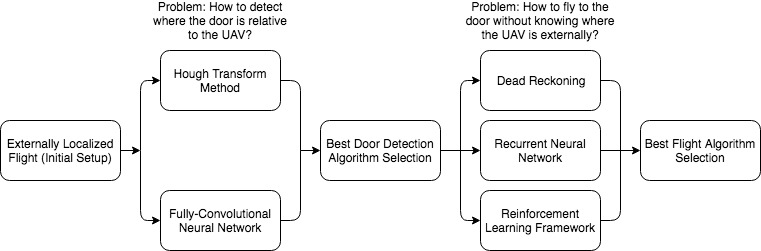
\includegraphics[scale=.55]{flowchart}
	\vspace{10pt}
	\caption[Flowchart of Proposed Development Stages]{Flowchart of Proposed Development Stages}
	\label{flowchart}
\end{figure}

%A background and summary of previous work in this area, along with an explanation that places the project in the context of what has been done before, and appropriate citations to peer-reviewed sources.
\section{Background}
Previous work in this area falls into a few broad categories. Detection of doors in camera images has been studied in multiple works and is a key initial step in flying through a door. Work in this category includes the detection of elevator doors by JunYoung and Lee \cite{ElevatorDoors} using stereo vision. While the current project will not use stereo vision, the corner detection JunYoung and Lee propose is used in later works. A more relevant publication is Mu\~noz-Salinaz et al.\cite{Fuzzy}, which used fuzzy logic to successfully detect doors using the edges present in an image including when the door is not completely visible. Tian \cite{Tian2013} attempts to expand on this concept and uses the detection of frame corners and edges to indicate a door, along with the heuristic that doors tend to be inset in the wall, while objects similar to doors such as wardrobes tend to extend out from wall. While this is useful for higher resolution cameras, the low accuracy of the camera proposed for this project may lead to an inability to extract enough corners and edges to determine if something is inset or standing out. Llopart, Ravn, and Andersen\cite{NNDoor} use a convolutional neural network to detect doors and cabinets. The network is trained to place a bounding box around any doors in a camera's image. The results show success, however, do not directly translate to the problem domain proposed here due to the high resolution and stationary nature of the camera in their work.


Indoor navigation of UAVs is a well-researched field. Most research focuses on either UAVs big enough to hold higher-accuracy sensors, or systems where the UAV is localized using motion capture setups such as VICON. Sanket et al. \cite{gapflyt} makes use of a UAV over ten times the weight of the Crazyflie to detect gaps and fly through them using Temporally Stacked Spatial Parallax, a gap detection method, and a high resolution camera-based approach. Their method is very successful for irregular gaps and proposes the use of a ``safe point'' that is chosen as the location to fly through the gap, calculated to ensure that the UAV will fit through the gap. Riviere, Manecy, and Viollete\cite{Folding} use a micro-UAV shaped like an `H' which is able to fold the H's uprights to form a flat body more able to fit through small gaps. A motion capture system is used to localize and control the UAV in this case. Horvath, Zentai, and Jenak\cite{PCNav} attempt to solve the problem of indoor navigation using a laser scanner capable of generating a three-dimensional point cloud combined with camera images. Their results are good for large spaces and varied environments but rely on the use of heavy sensors. Barrows\cite{crazyflie_centeye} uses new, extremely small-scale stereo optical flow sensors to detect objects and maintain position without an external localization system. The hardware is not available commercially, and the work does not indicate that these sensors can be used to actually navigate as opposed to simply hold position or avoid obstacles. 

%A detailed description of the project, updated as appropriate.
\section{Project Description \& Progress}
\subsection{Hardware and Pre-existing Software}
The UAV selected for this project is the Crazyflie micro-UAV, shown in Figure \ref{crazyflie_image}. Developed by Seeed Studios, it has a built-in IMU and a 15 gram payload. This payload will consist of an FPV camera weighing 5.6 grams manufactured by RunCam, shown in Figure \ref{crazyflie_cam}. This device has a global shutter which negates the distortion caused by rolling shutter cameras. Under rapid motion, rolling shutter cameras produce very distorted images because they scan line by line. The top of the image is captured at a different time and location from the bottom, producing undesirable smudging of objects in the image. The global shutter avoids this effect. An analog video transmitter and originally a separate battery to power the camera/transmitter combination formed the rest of the payload. Combined with the UAV's battery, the weight of the payload caused flight instability during initial test flights in many configurations. The high center of gravity caused the UAV to gather momentum from small perturbations during level flight and flip over. A new payload system (Figure \ref{payload}) has been created over the last few months. The design places the camera in a protected enclosure below the main UAV body. The stock battery has also been replaced with a lighter battery of similar capacity and wiring harness modified to allow both the UAV and camera/transmitter combination to run from the same battery. These changes have resulted in a configuration that meets the UAV's takeoff weight requirements and can fly to waypoints in a motion capture system.

\begin{figure}
    \centering
    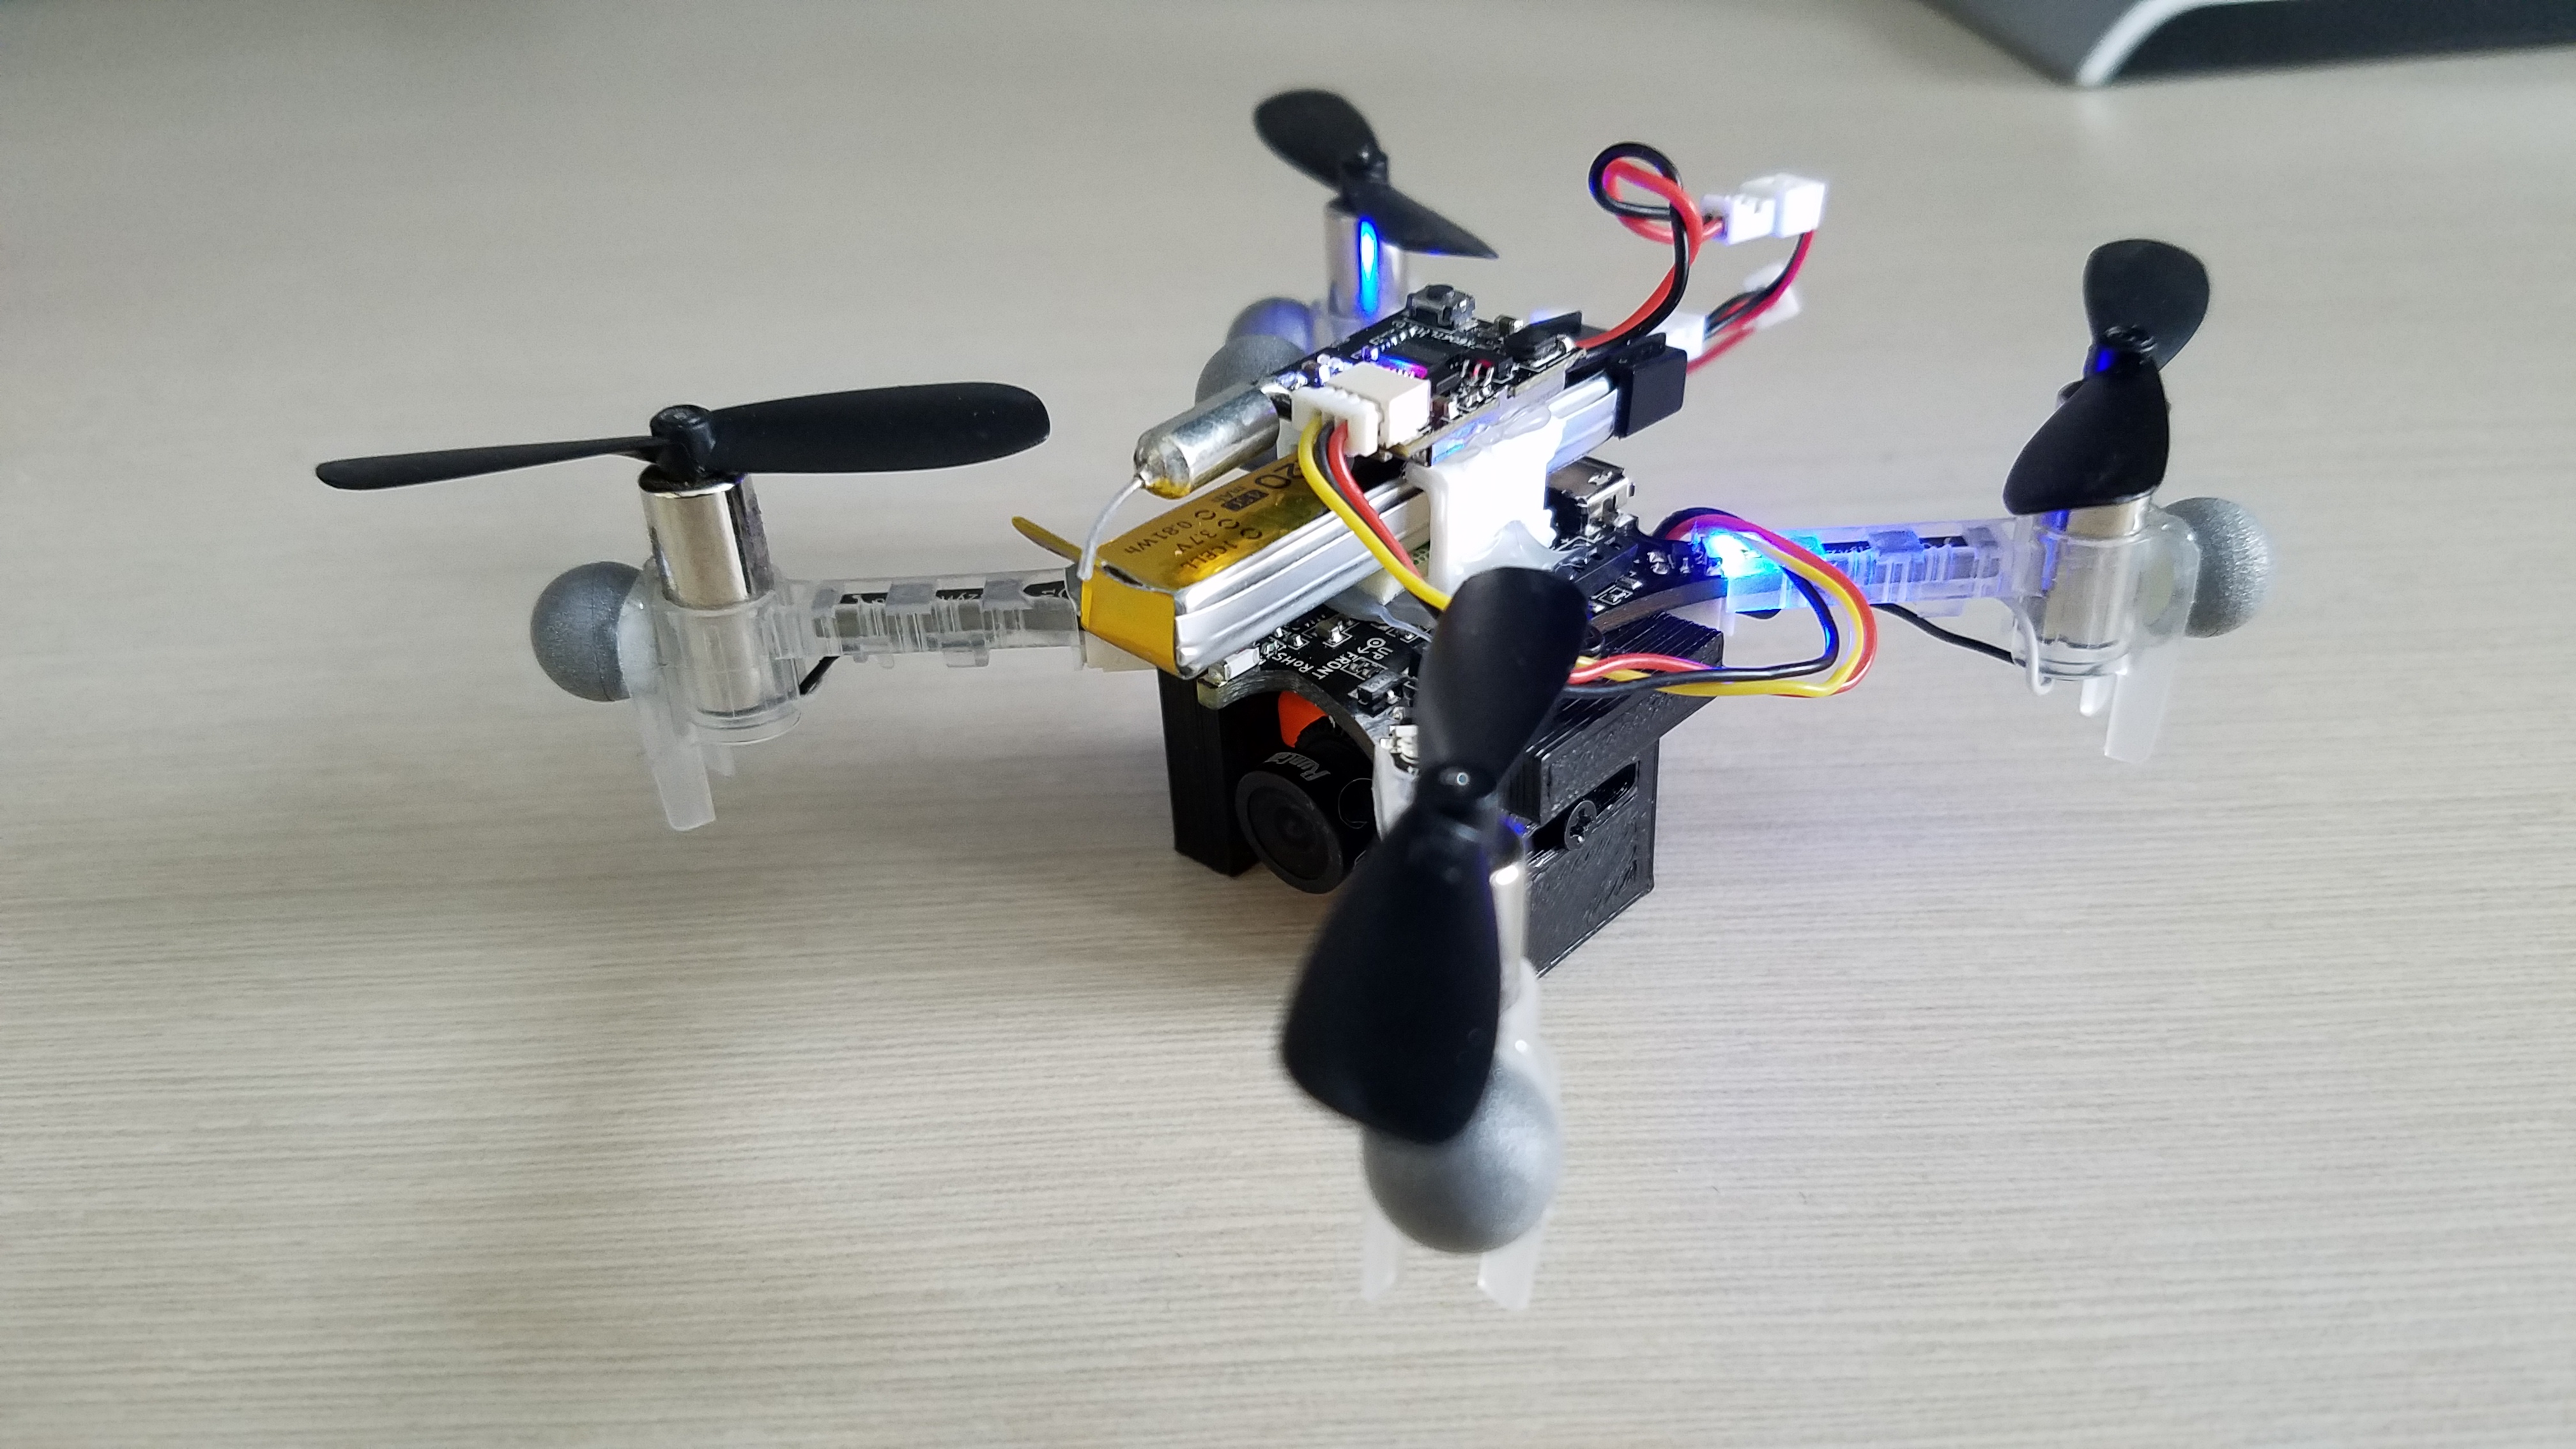
\includegraphics[scale=0.075]{payload1}
    \vspace{10pt}
    \caption[Newly developed UAV payload]{Newly developed UAV payload}
    \label{payload}
\end{figure}

In order to provide ground truth to test against, a motion capture system developed by VICON will be used. By placing lightweight plastic balls in unique configurations on the UAV, the system tracks the full three-dimensional poses of the UAV to an extremely high degree of precision using many cameras. This will be used as a ground truth source and as a next step after simulations to verify that a portion of the algorithm works reasonably. For example, the door-detection methods can be run during flight without the non-external navigation software being written. In this way, the development of individual parts of the project can be decoupled from each other. The UAV communicates with the ground station (a basic laptop) through two radio links: a two-way link for UAV commands and basic sensor data streams and a separate link for camera image data to reduce latency on both links.

\begin{figure}
	\centering
	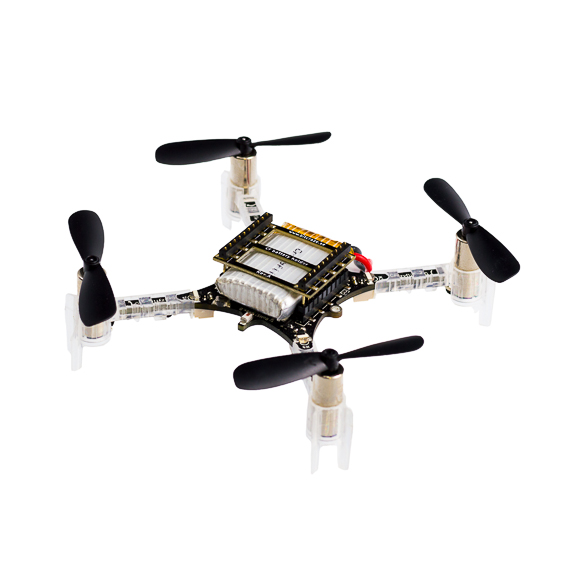
\includegraphics[scale=1.7]{crazyflie_new}
	\caption[The Crazyflie micro-UAV]{The Crazyflie micro-UAV}
	\vspace{8pt}
	\small Source: \url{https://www.bitcraze.io/crazyflie-2/}
	\label{crazyflie_image}
\end{figure}



\begin{figure}
	\centering
	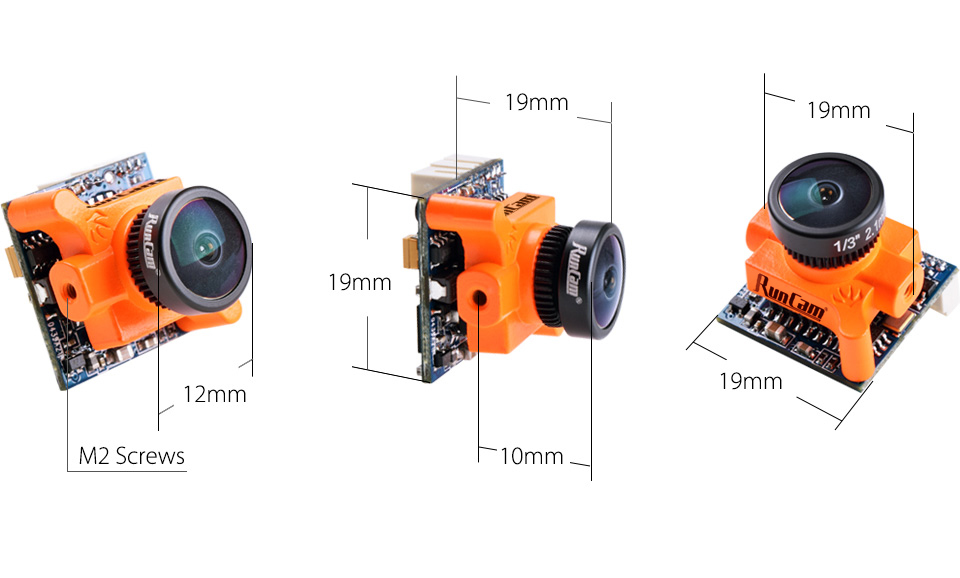
\includegraphics[scale=0.3]{micro-swift-size}
	\caption[The RunCam Micro Swift Camera]{The RunCam Micro Swift Camera}
	\vspace{8pt}
	\small Source: \url{https://shop.runcam.com/runcam-micro-swift/}
	\label{crazyflie_cam}
\end{figure}

In order to control the UAV, the Robotic Operating System (ROS) will be used. ROS allows communication between running processes creating greater modularity in code. Processes become ROS nodes which each can handle a different aspect of robotic control. A node for interacting with the Crazyflie, called \verb|crazyflie_ros|\cite{crazyflie_ros}, exists and implements several important features. It allows complete waypoint navigation of the UAV when used with a motion capture system to localize the UAV, and generally handles much of the low level UAV control. Without a motion capture system, the node uses the onboard IMU and motor PWM frequencies to respond to pitch, roll, yaw, and thrust level commands from other ROS nodes. This node has been tested and functions well in both regimes.

The camera attached to the UAV will be forward facing with the lens pointing out along the UAV's x-axis. The camera-UAV transform has been calibrated for more precise measurements due to the impossibility of perfect camera mounting by a human. Given the assumption of the IMU as the ``center'' of the UAV, which for the Crazyflie is sufficiently close to true, the motion of the camera and the IMU can be correlated to determine how they are related spatially. This has been done with Kalibr\cite{Kalibr}, a calibration toolbox developed by ETH Zurich. The camera itself has also been calibrated using the same package. The \verb|image_undistort| \cite{image_undistort} node, also from ETH Zurich, has been set up to perform undistortion of the images coming from the UAV in real time using the performed calibration. 

In order to speed development and allow verification of code in a safe and easy way, code will first be tested in simulation where possible. The environment chosen for this is the Virtual Robotics Experimentation Platform, or V-REP, developed by Coppelia Robotics. A room with a door has been created in simulation, along with a UAV matching as closely as possible the characteristics of the Crazyflie. The ROS interface provided by V-REP will be used to send commands in a format identical to what \verb|crazyflie_ros| expects, and will output IMU and camera data in the same format as \verb|crazyflie_ros| does as well. In order to replicate the real-life environment more precisely, the IMU data generated by V-REP has artificial noise added to it, and the camera data is lowered in resolution and noise added. Both data streams have delays associated with them as well in order to mimic the latency of the data links in real life. Functionality usually provided by a motion capture system, such as precise localization of a target object, is easily achieved in the simulation and can be output in the same format as the motion capture system does.

\subsection{Externally Localized Flight}
The first part of the project focused on ensuring the stability of the UAV's flight and doing initial setup of systems. A simulation was set up which broadcasts the location of the UAV and door in a common reference frame. A node was implemented to run waypoint navigation through the door using these broadcast locations, which will be used as the ground truth for how the UAV will fly. The same node will be used to fly in the motion capture system, since the system provides the same location broadcasts as the simulation. Final test flights have been completed, meaning everything is ready to run this node in the VICON space to test its real-life functionality. Success in this stage is defined by safely flying through the doorframe and landing while not running out of battery mid-flight. 

\subsection{Image Based Door Detection + Externally Localized Flight}
In the next portion of work, the need to automatically detect where the door is using the UAV camera, not the motion capture system, was explored. Software was written which is able to determine where in the UAV's camera image it thinks a door is visible. This software takes an image as input and outputs the $(x,y)$ coordinates it considers to be the middle of the door. The door must be correctly identified with a high success rate in order to make the entire project succeed. It must perform this correct identification under many environments, as the door will not always be placed directly in front of the UAV with a clear distinction between door and surrounding wall. The door might appear very different due to the UAV's perspective and could be only partially visible during some stages of the UAV's flight, such as when it approaches very close to the door. Door detection was achieved in multiple ways: through a method relying on the Hough transform to find door frame edges in the image, and through a convolutional neural network.

\subsubsection{Hough Transform-Based Method}
In the Hough-based method the camera image, once received, is converted to grayscale. After bilateral filtering, the edges in the $x$ and $y$ directions of the image are detected using a Canny edge detector. These edges are then thresholded to select only the strongest edges which might be the door frame. The edges are then converted into the Hough space. To do this, each pixel in the image has several lines associated with it, specifically ones which are firstly perpendicular to rays leaving the image origin and secondly pass through the point. A ``vote'' for this associated line will be recorded. The lines with a number of votes above a threshold will be selected as lines in the image. Significant filtering of the resulting lines is done to reduce the effects of image noise and multiple detections of the same line. Lines which are relatively parallel (within a small angle of each other) are grouped together using a k-means clustering. This results in two groups of lines, one going vertically and the other horizontally. The intersection point of the lines within each group is then calculated and treated as a vanishing point of the image. Since we expect there to be a door in the image this assumption of two vanishing points should hold. The vanishing points are used to construct a vanishing line which is used to rectify the image to be fronto-parallel to the camera. The fronto-parallel view is a transformation of the image so it is taken with the camera on the normal of the plane the door lies in. The door should have a consistent aspect ratio in this view. The same transform is used on the detected sets of lines. Rectangles in the set of lines are then generated, and the largest which matches the standard door aspect ratio is selected as the door. The center of this rectangle is output as the result (after inverse transforming it back into the original view). Due to noise and motion blur, reasonable vanishing points cannot always be determined. Since the previously described sequence depends on the points to rectify the image and determine the door rectangle, a tracker was introduced to allow a reasonable door center to be output when the image could not be rectified. A tracker using Kernelized Correlation Filters \cite{KCF} was selected for its high-speed yet accurate performance on image streams where the object might be occluded. This tracker is re-initialized whenever an image is able to be rectified, and tracks the pixels in the last determined door rectangle otherwise. This approach suffers from the fact that this process is lengthy and possibly slow, meaning it cannot run in real-time. Additionally, when the UAV moves very quickly the tracker is unable to keep up with the door moving so fast in the image, and can lose tracking in this way. If a full view of the door is not seen for a little while the tracker is also not re-initialized and loses accuracy over time. 

\subsubsection{Convolutional Neural Network Method}
The second door detection method uses a neural network to determine the center of the door in the image. The architecture chosen for this task uses the image as input, passes it through several convolutional layers (each of which is followed by a max-pooling operation), after which the last layer is fed through a fully-connected layer with two outputs: the $x$ and $y$ coordinates of the door center. This architecture (as seen in Figure \ref{arch}) was chosen due to its small size since it will be running on the UAV ground-station which has limited resources. The network is built and trained using Keras with a Tensorflow backend, a high-level interface for machine learning. The training data was collected using the UAV's camera filming a doorframe constructed from wood. The number of convolutions learned at each level is much smaller than in related networks such as in \cite{NNDoor}: just 8,then 16, then 32. This also speeds processing of each image. After training, it became evident that the dataset contained a bias, with most views having the door in the relative center of the image. It is thus likely that the network simply learned to select a point near the middle of the image that was the color of the wall behind the doorframe. The dataset was augmented through translational and rotational transforms to remove this bias. The retrained network did not perform nearly as well on a either the training or a novel validation dataset. Since the size of the network is likely playing a role in its inability to learn the center of the door, larger networks are currently being trained to perform similar detection. Originally, U-net \cite{Unet} was selected, but the large size of the network led to unacceptably slow inference speeds. Thus, much leaner networks like MobileNet \cite{howard2017mobilenets} and Tiny YOLOv3 \cite{yolov3} were selected for testing. The last few layers of each of these networks were removed since they output results as bounding boxes instead of the desired $x$ and $y$ door center coordinates. These layers were replaced with a fully connected layer leading to two outputs, i.e. the $x$, $y$ door center coordinates. Currently, all networks were trained on a single dataset. A future step might be to train the network on a larger dataset of doors, such as those from MIT's CSAIL\cite{csail_data_2}\cite{csail_data_1}.


\begin{figure}
	\centering
	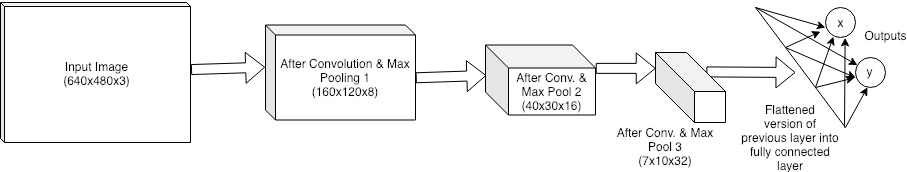
\includegraphics[scale=0.5]{arch}
	\caption[Sample door detection network architecture]{Sample door detection network architecture}
	\vspace{10pt}
	\label{arch}
\end{figure}

\subsubsection{Comparison Techniques and Other Considerations}
Since with a single camera it is impossible to estimate the distance to the door, the door center in the image will simply provide a unit vector in the direction the UAV should fly in the camera's frame of reference. By using the camera-UAV transform determined previously, the UAV would then be able to determine the direction it should travel to make it through the door by chaining transforms. The error of a detection can be calculated by the euclidean distance from the detection to the ground truth center of the door. Success in this stage is defined as one of the methods compared achieving an average error of less than 30 pixels across a test set of images. In order to calculate this score and compare the different methods, a sample video has been taken of a door with the UAV's camera. The video has been hand-annotated with the correct location of the door center in each frame. The detection results of each method is then compared frame by frame with the annotated ground truth and an average error calculated. In addition to error rate, the speed of the method is a key factor. The UAV provides images at about 30 frames per second (fps), and previous experience suggests that a control loop for the UAV must run at at least 10 Hz. The best method must thus also be able to run ideally at least at 30 Hz, in order to process each frame in time for the next one and to give some time for the control loop code to run so it can achieve 10 Hz. Below are the results of a preliminary comparison between the Convolutional Neural Network and the Hough Transform method:

\begin{table}[H]
\begin{tabular}{lll}
\begin{tabular}[c]{@{}l@{}}\end{tabular} & Hough Method   & Convolutional Neural Network \\
Mean sec/image                                                     & 0.254314567058 & 0.0239195841163              \\
Std. dev. sec/image                                                & 0.261605686471 & 0.00660748004691             \\
Mean Accuracy                                                      & 73.6029293414  & 36.2429306581                \\
Std. dev. Accuracy                                                 & 67.5749586736  & 25.5508142198
\end{tabular}
\end{table}

The accuracy data here is somewhat unfair to the Hough Method, as the dataset used to generate these statistics was the same as the one used to train the network. The network performs far worse when tested on another dataset. The neural network is, however, an order of magnitude faster than the Hough transform based method. The speed difference is likely due to the large amount of processing that the Hough method performs, while the network is in essence optimized for the door detection task and does not generate extraneous information. This could likely be remedied through some code optimization that will be done in the near future. The larger networks currently being trained are expected to still be much faster than the Hough Method. A future step will be running the same experiment as above on a new and larger dataset, in order to remove the advantage the network had in this experiment. This will allow a true comparison of both methods. A final step is to have the UAV navigate to the door using the VICON system for movement and motion control but using its onboard cameras to determine a direction to travel.

\subsection{Image Based Door Detection + Independent Flight}
The final portion of the work will remove the motion capture system entirely from the equation, requiring the UAV to fly without outside knowledge of its orientation and location. In place of the motion capture system, the onboard IMU and camera will be used to both keep the UAV stable and provide information about how the UAV is currently flying. A series of pitch, roll, yaw, and thrust commands will be generated constantly, and the UAV will need to execute them with feedback from the sensors to fly through the door. The motion capture system will likely still be used as a safety backup and ground truth, but this information will not be fed into the nodes used by the UAV for any task. Three different systems will be developed and tested to see their effectiveness at successfully having the UAV fly through the door. The first is a simple technique where the UAV simply tries to fly open-loop towards the door. The second is a recurrent neural network (RNN) technique, which has several variations but will use the IMU output, the camera image, and possibly the detected center of the door to generate a stream of commands after having been trained. Finally, a reinforcement learning (RL) system is proposed which will use a multi-factor metric as a reward signal to train a neural network to generate the command sets. 

\subsubsection{Dead Reckoning}
The first approach will be a dead-reckoning system, which initially has access to the position of the door and the UAV's initial location from the motion capture system. It determines a vector between the UAV and the door and flies along it until it makes it through the door. This algorithm has been simulated, and will shortly be flown in real life. The second step to this method will remove the dependence on the motion capture system and replace it with the information from the detected door. After taking off and beginning to fly toward the door, it will attempt to correct any drift that occurs by using the motion of the door in the camera image as a measure of error. Corrections will be made to minimize the movement of the door in the image frame, thus leading to the UAV flying through the door as long as it is flying towards the door initially. This method will depend on getting a consistent detection throughout the flight.

\subsubsection{Recurrent Neural Network}
The second approach uses an RNN trained to navigate through the door using simulation and afterwards the motion capture system to provide ground truth using methods described by Kelchtermans and Tuyelaars\cite{RNNTraining}. The RNN will be built using Python's Tensorflow library. An RNN is a good choice for this task since it has some level of memory, allowing it to handle velocities during flight. Using the flight method described in the initial section on externally localized flight, the UAV will be flown repeatedly in simulation from random starting locations with various door configurations. The RNN will train based on the IMU and camera data generated during these flights. Tests will then be performed on how well the network is able to provide correct command sets to the simulated UAV so that it flies through the door. Several variations are proposed. One uses the unmodified camera feed to train the network. Another instead uses the results of one of the door detection algorithms as the input instead of full camera images. Finally, the output of the network may be designed to select an action out of a limited, discretized action space instead of outputting a continuous set of roll, pitch, yaw, thrust UAV control inputs. These discretized actions may be things such as ``increase thrust by a factor of 2'' or ``fly to the right.'' If these tests are successful, the same network will be re-trained with the real UAV, using the motion capture system to do the ground truth control of the UAV. Ideally the network will not have to be entirely retrained, only modified to deal with the real-life dynamics of the Crazyflie, what the test door looks like, and the real-life IMU.

\subsubsection{Reinforcement Learning Neural Network}
An RL framework approach will also be attempted in order to fly the UAV without any outside source of information such as the motion capture system. In order to train an RL network, a reward signal is needed which allows the network to infer how well it is performing without supervision. The proposed signal is a weighted sum of how close to the door the UAV is ($D$), how within a reasonable range the current UAV pose is, i.e. the UAV is not upside down, ($R$), how close it is to obstacles such as the ground, walls, and doorframe ($O$), and possibly other factors. The higher the reward signal, the better the network is performing. The signal might take the form of something like:
$$
Reward = K_{1}/D + K_{2}*R + K_{3}*O + K_{n}*OtherFactors
$$

Using the openAI Gym framework and A V-REP simulation, the RL network is currently being trained similarly to the RNN in simulation. A system which calculates the reward signal was created and the network designed to use the IMU and camera data to predict the command set inputs. The flight of the UAV is again being simulated repeatedly. However, there is no ground truth being provided to teach the network by the simulation. Instead, it attempts to maximize its reward signal through different actions. Eventually this should lead to a network which is able to successfully navigate through the door. If successful, the same technique will be used in real life with the motion capture system. The data from the motion capture system will be used to generate the reward signal. Ideally the network will be mostly trained in simulation and only require a small re-learning period in real life, in order to minimize the number of flights that have to be set up by hand. The setup for this portion of the work has been completed. In the next stages, a network architecture will need to be selected, some remaining bugs removed, and the network trained.

\subsubsection{Comparison Techniques and Other Considerations}
Upon developing, testing, and comparing these three systems, the best will be chosen. Success in this stage will indicate the goals of the entire project being achieved, with the UAV able to start from a random initial location, detect and fly through the door, then land safely on the other side. The methods proposed will be compared in simulation first. Each will be run 100 times in simulation with a random initial location. The number of times the method succeeds in flying the UAV through the door, defined as traveling through the doorframe and landing with the propellers facing up, will be used as the method's score. In real life a similar comparison will be run. The most successful method will be the one that has the highest score in real life. Success for this project will be defined as a less than 20\% failure rate for flying through the door with at least one of the methods mentioned in this section. 



%h) Budget - Funds needed to perform the studies.
\section{Budget}
The twenty (20) dollar budget was used to build the physical doorframe which the UAV will fly through when flying within the motion capture system. 

%An update of the expected timeline.
\section{Timeline}
\begin{itemize}
    \item \sout{Sep 17 - Simulation setup completed}
    \item \sout{Sep 29 - UAV calibration complete}
    \item \sout{Oct 08 - Project Proposal complete and submitted}
    \item \sout{Oct 15 - Initial full motion capture setup and successful test flight with human control}
    \item \sout{Oct 19 - Full external localization navigation node written and tested in simulation}
    \item \sout{Oct 25} Feb 15 - Full external localization navigation node tested in real life
    \item \sout{Nov 02 - Hough transform based door-detection node written and tested in simulation and real life}
    \item \sout{Nov 30 - Neural network door-detection node written and tested in simulation and real life}
    \item \sout{Dec 12 - Full comparison run between door-detection nodes, best one determined}
	\item Feb 01 - Progress Update complete and submitted
    \item Feb 10 - Hough transform node speed optimized
    \item Feb 15 - Door detection comparison run on novel dataset
    \item Feb 28 - Dead reckoning navigation node written and tested in simulation and real life
	\item Mar 15 - RNN navigation node written and tested in simulation and real life
	\item Mar 30 - RL navigation node written and tested in simulation and real life
	\item Apr 05 - Navigation nodes compared and best one selected
	\item Apr 29 - Project complete
	\item May 10 - Project Report complete and submitted
\end{itemize}

%j) Conclusion/Summary – A succinct summary of your proposed project.
\section{Conclusion}
In conclusion, this project seeks to explore the applicability of various techniques and approaches to indoor navigation by very small UAVs. To do this, a specific problem is defined: navigating from an arbitrary initial position through a doorway and landing safely on the other side. The sensing package defined is purposely limited to low-cost, low-quality, and relatively high-latency sensors on an extremely small platform in order to explore how navigation and motion might be controlled in extremely limited environments. To this end, a Crazyflie micro-UAV with a low-resolution camera is selected as the platform for experiments. To complete the task, several discrete pieces of software have been/will be written and connected through the Robotic Operating System. The first is a door-detection algorithm. Several options for this algorithm have been explored including a Hough transform-based algorithm and a convolutional neural network. Next, a way to navigate without any external localization systems will be written. This will likely depend on the IMU internal to the UAV and possibly on the camera image. Several options for this will also be developed and tested against one another, including a simple dead reckoning system, a recurrent neural network, and a reinforcement learning network (already under development). To speed development, each of the above steps will first be implemented in a V-REP simulation. Once they are successful in simulation, the software nodes written will be transferred to the real life system, which will be flown in an environment monitorable by a motion capture system. This system will allow training of algorithms that require a ground truth and act as a safety net, stopping the flight of the UAV if it is determined to be out of control.
%k) List of References - Numbered list of references that must include for each reference: authors, title,
%name of the source (e.g. conference, journal, etc.), and date of the publication. You should use the
%citation format that is standard for the primary journals in your specific field of research.
\bibliographystyle{plain}
\bibliography{../../references}

%Written project proposals are typically about 10 to 12 double-spaced pages in length for the main text
%and figures, but excluding the title page, abstract, table of contents, list of figures, budget, timeline, and
%references. They should be in 12-point font with one-inch margins. Introduction(1) + Background(1.5) + Proposed Project(7) + Conclusion(1) is 10-12 pages


%The oral project proposal presentation will give you the opportunity to describe your ideas and to show
%the soundness of your proposed approach to your peers, your project advisor, and the course coordinator.
%This presentation should include all of the above components. Your project proposal presentation should
%be 10 to 12 minutes long, followed by 3 minutes for Q&A.
\end{document}
